\documentclass{standalone}
\usepackage{pgfplots}
\pgfplotsset{compat=1.17}

\begin{document}
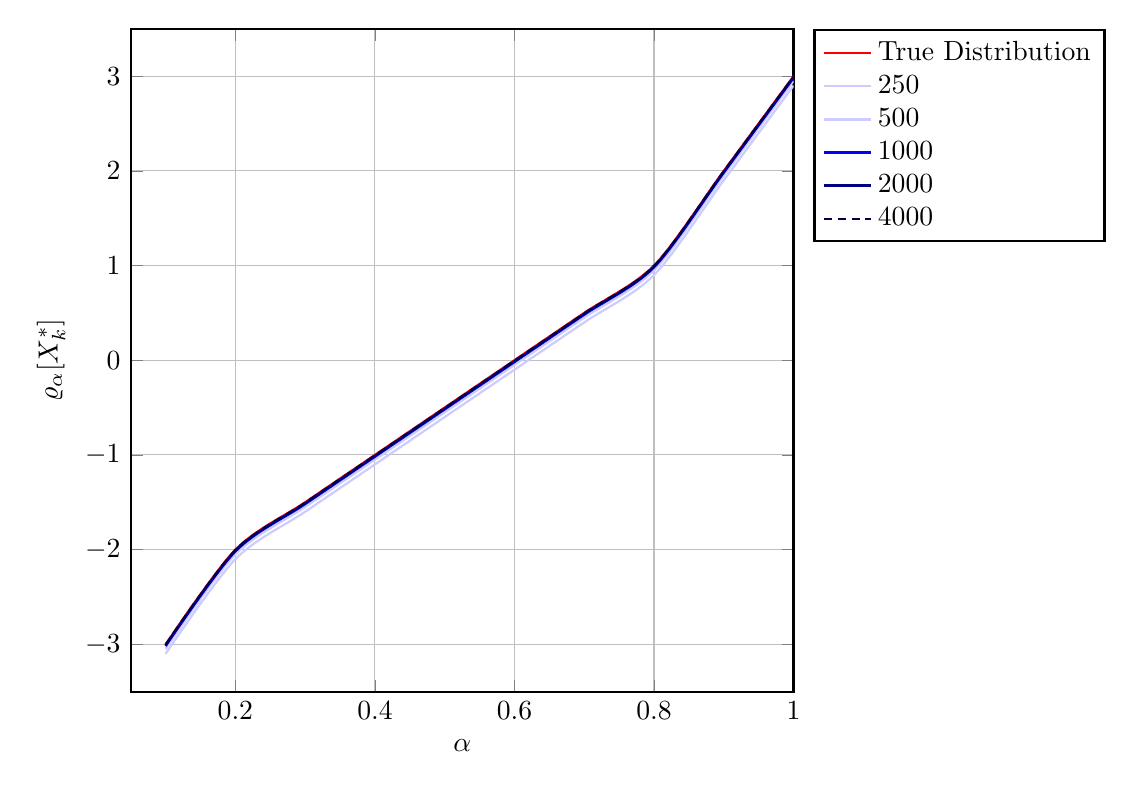
\begin{tikzpicture}
\begin{axis}[
    xlabel={$\alpha$},
    ylabel={$\varrho_{\alpha}[X^{*}_k]$},
    xmin=0.05, xmax=1,
    ymin=-3.5, ymax=3.5,
    legend pos=outer north east,
    legend cell align={left},
    grid=major,
    smooth,
    thick,
    width=10cm,
    height=10cm,
]

% True distribution (red line)
\addplot[red, thick] coordinates {
    (0.1, -3.0)
    (0.2, -2.0)
    (0.3, -1.5)
    (0.4, -1.0)
    (0.5, -0.5)
    (0.6, 0.0)
    (0.7, 0.5)
    (0.8, 1.0)
    (0.9, 2.0)
    (1.0, 3.0)
};

% Simulated distribution (blue lines for different sample sizes)
% Note: These are example coordinates; you might need to adjust them to match the image exactly.
\addplot+[blue!20, mark=none] coordinates {(0.1, -3.1) (0.2, -2.1) (0.3, -1.6) (0.4, -1.1) (0.5, -0.6) (0.6, -0.1) (0.7, 0.4) (0.8, 0.9) (0.9, 1.9) (1.0, 2.9)}; % 250
\addplot+[blue!20, mark=none] coordinates {(0.1, -3.05) (0.2, -2.05) (0.3, -1.55) (0.4, -1.05) (0.5, -0.55) (0.6, -0.05) (0.7, 0.45) (0.8, 0.95) (0.9, 1.95) (1.0, 2.95)}; % 500
\addplot+[blue, mark=none] coordinates {(0.1, -3.02) (0.2, -2.02) (0.3, -1.52) (0.4, -1.02) (0.5, -0.52) (0.6, -0.02) (0.7, 0.48) (0.8, 0.98) (0.9, 1.98) (1.0, 2.98)}; % 1000
\addplot+[blue!50!black, mark=none] coordinates {(0.1, -3.01) (0.2, -2.01) (0.3, -1.51) (0.4, -1.01) (0.5, -0.51) (0.6, -0.01) (0.7, 0.49) (0.8, 0.99) (0.9, 1.99) (1.0, 2.99)}; % 2000
\addplot+[blue!30!black, mark=none] coordinates {(0.1, -3.005) (0.2, -2.005) (0.3, -1.505) (0.4, -1.005) (0.5, -0.505) (0.6, -0.005) (0.7, 0.495) (0.8, 0.995) (0.9, 1.995) (1.0, 2.995)}; % 4000

\legend{True Distribution, 250, 500, 1000, 2000, 4000}
\end{axis}
\end{tikzpicture}
\end{document}